\setlength{\parskip}{1pt} %% ESPAÇO DEPOIS DE 6pt
\pagenumbering{arabic}  %% PAGINAÇÃO INICIA AQUI
\setcounter{page}{16} % Reiniciar contagem de página para 1
%\pagestyle{plain} % Restaurar numeração de página com estilo "plain"
\clearpage
\pagestyle{fancy}




\section{Introdu{\c c}{\~a}o} \label{sec:int}



No âmbito da demanda d'água, desempenha-se um papel crucial nesse contexto. A água está presente em todos os aspectos do cotidiano, sendo essencial tanto para atividades básicas, como o banho, quanto para o consumo. A compreensão da importância desse recurso é vital, uma vez que ele influencia diretamente a qualidade de vida em várias esferas.
Existem três tipos principais de Aprendizado de Máquina: Supervisionado, Não Supervisionado e por Reforço. No Aprendizado Supervisionado, é necessário apresentar a resposta desejada para cada exemplo. No Aprendizado Não Supervisionado, os exemplos são fornecidos sem rótulos, sendo agrupados por similaridades. No Aprendizado por Reforço, o algoritmo recebe sinais de reforço, sem a resposta correta, e determina a eficácia de suas hipóteses \cite{Silva2021}.

Nesse caso, os modelos usados nessa dissertação são os modelos de aprendizado de máquina supervisionados. Esses modelos para série temporal são usados na literatura.
As séries temporais são caracterizadas como processos estocásticos regidos por leis probabilísticas.
Série estacionária com média é aquela que contém a média, variância e autocorrelação constantes ao longo do tempo.

A abordagem desse estudo envolve o problema de abastecimento d'água que afetou a cidade de Curitiba no Bairro Alto entre os anos de 2018 e 2020. Durante esse período, os habitantes enfrentaram a escassez de água, sendo necessário implementar rodízios, alternando períodos com e sem fornecimento. Os dados utilizados foram coletados pela companhia de saneamento do Paraná (SANEPAR).


A previsão da demanda de água ao longo do tempo é essencial para um planejamento sustentável e eficiente do abastecimento hídrico, especialmente no contexto urbano, como é o caso da cidade de Curitiba, no estado do Paraná. Neste estudo, adotou-se alguns modelos de previsão da área de aprendizado de máquina e o modelo clássico ARIMA (\textit{Auto-Regressive Integrated Moving Average}) para realizar previsões diárias da demanda de água ao longo do tempo.

Os modelos de aprendizado de máquina foram aplicados na previsão de séries temporais com dados coletados pela SANEPAR. Cada modelo tem suas particularidades, mas os modelos de aprendizado de máquina podem ser otimizados da mesma forma que os modelos clássicos do tipo ARIMA e RNN (\textit{Recurrent Neural Network}). Os dados coletados pela SANEPAR, utilizados para previsão, referem-se ao abastecimento d'água no Bairro Alto durante o período de 2018 a 2019.


Por meio da utilização de métodos e modelos de séries temporais, realiza-se a previsão do nível do reservatório (LT01), incorporando diversos modelos nesse processo. Dentre esses modelos, incluem-se os clássicos, como ARIMA e suas variantes, tais como AR (do inglês \textit{Auto-Regressive}), ARX (do inglês \textit{Auto-Regressive with Exogenous input}), MA (do inglês\textit{Moving Average}), ARMA (do inglês \textit{Auto-Regressive Moving Average}), SARIMA (do inglês \textit{Seasonal Auto-Regressive Integrated Moving Average}), ARIMAX (do inglês \textit{Auto-Regressive Integrated Moving Average with Exogenous input}), SARIMAX (do inglês \textit{Seasonal Auto-Regressive Integrated Moving Average with Exogenous input}), Prophet, além dos modelos de aprendizado de máquina, como árvore de decisão, floresta aleatória, XGBoost (do inglês \textit{Extreme Gradient Boosting}), Light GBM (do inglês \textit{Light Gradient Boosting Machine}), e redes neurais como LSTM  (do inglês \textit{Long Short-Term Memory}), GRU (do inglês \textit{Gated Recurrent Unit}), RNN, Transformer, CNN (do inglês \textit{Convolutional Neural Network}), ANN (do inglês \textit{Artificial Neural Network}). A diversidade de abordagens busca otimizar a precisão das previsões, destacando a abrangência e sofisticação desse trabalho.


\subsection{Contexto da Pesquisa} \label{subsec:contexto}

Torna-se evidente que a análise de séries temporais e previsões são ferramentas valiosas para apoiar o processo de tomada de decisão em curto, médio e longo prazo. Devido às não linearidades, sazonalidades e tendências que podem ocorrer nos dados temporais de abastecimento de água, o desenvolvimento de modelos de previsão eficientes torna-se uma tarefa desafiadora \cite{mateus}.

Na Figura \ref{fig:paradigma-ml}, as etapas de como a análise de dados e a seleção dos modelos devem ocorrer são apresentadas. Essa escolha pode ser conduzida de modo a determinar o que deve ser previsto na variável. Feito isso, a primeira etapa envolve a preparação dos dados, garantindo que cada um tenha sido identificado com seus rótulos de entrada e saída. É imperativo que os dados não contenham \textbf{NaN} (do inglês \textit{not a number}) ou dados ausentes, evitando assim falsos positivos.

\begin{figure}[!htb]
	\centering
	\caption{Paradigma de aprendizado de máquina}
	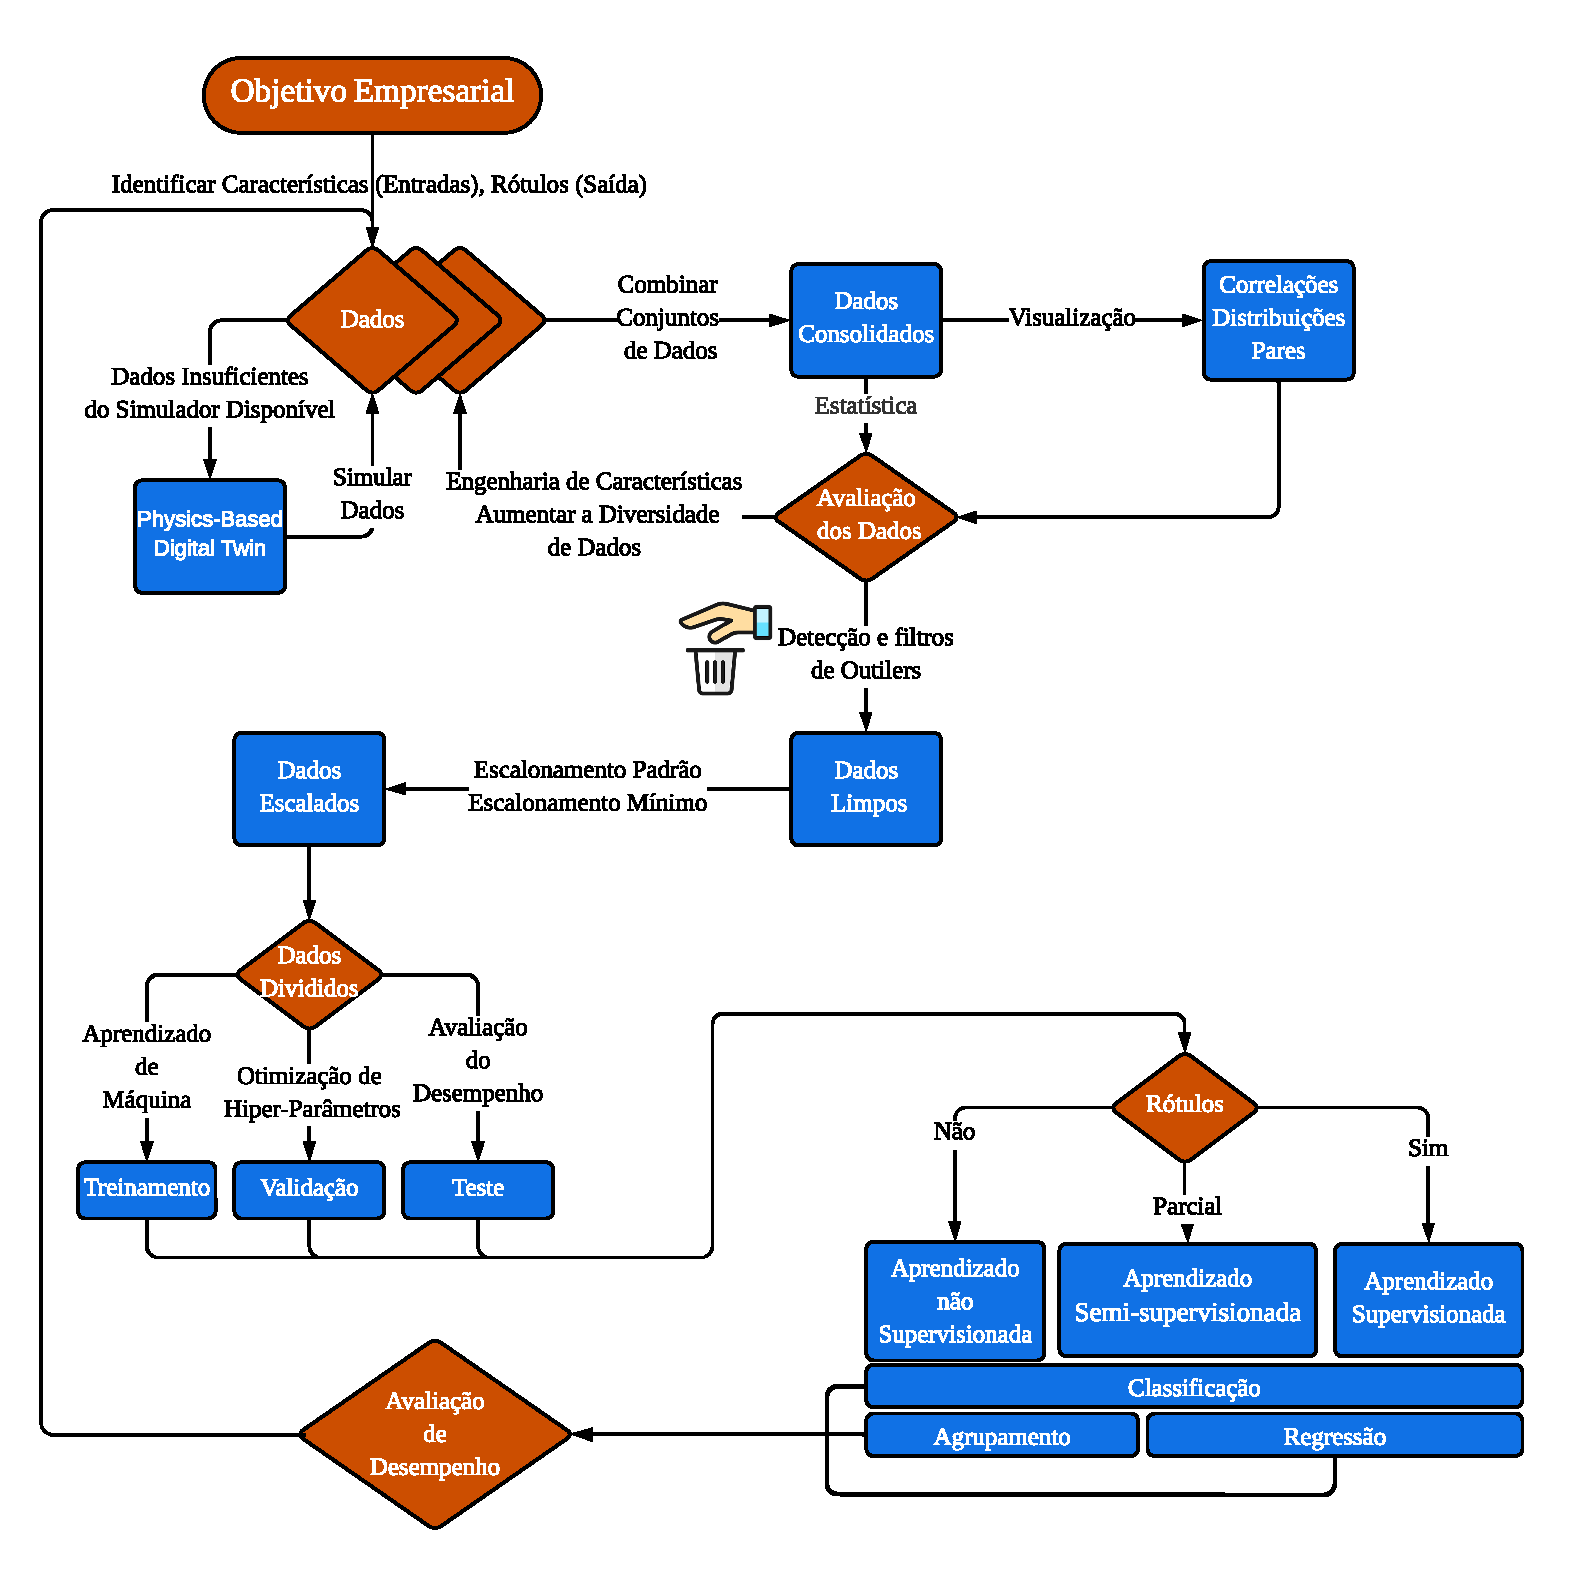
\includegraphics[width=\linewidth]{Introducao/Figuras/paradigma-ml}
	
	\fonte{Adaptado de \cite{apmonitor}}
	\label{fig:paradigma-ml}
\end{figure}

Ao realizar essa etapa, deve visualizar os dados para garantir que estejam carregados corretamente e em um tamanho tolerável, o que é conhecido como avaliação dos dados. Uma vez que os dados estejam limpos e devidamente carregados, sem falsos positivos, a divisão dos dados pode ser efetuada.
A otimização dos dados para os modelos pode ocorrer de diversas maneiras, como a utilização da biblioteca Optuna em Python, que emprega a otimização Bayesiana para cada modelo pré-listado, reduzindo assim o tempo de processamento.

A validação é uma prática comum em conjuntos de dados extensos, permitindo que os modelos interajam mais eficientemente com os dados e proporcionem resultados mais precisos. Após essa etapa, na escolha dos modelos, há a possibilidade de determinar se o modelo é de série temporal, classificação, agrupamento ou regressão. Posteriormente, ao listar os modelos, cada um deles deve passar por uma avaliação com métricas específicas para verificar a precisão de seus resultados.


\subsubsection{Motiva\c c\~ao da Pesquisa} \label{subsubsec:motivacao}

A motivação desta pesquisa baseia-se na situação enfrentada por Curitiba e região metropolitana, conforme destacado por \cite{vasconcelos_2020}. A região passou por um rodízio de abastecimento de água, com períodos de 36 horas com abastecimento de água, seguidos por 36 horas sem abastecimento. A média geral dos reservatórios na região estava em torno de $27,96\%$ de sua capacidade. Além disso, a quantidade de chuva nos anos anteriores, em $2020$, foi de $1.704$ mm, superando a média anual de precipitação de $1.490$ mm.

Diante dessa situação, a pesquisa tem como abordagem principal a previsão do abastecimento de água, associada a condições de seca ou decorrentes das consequências da COVID-19. A partir dos dados coletados pela SANEPAR, é possível realizar uma análise detalhada, com o objetivo de prever e evitar a ocorrência de escassez de água. 



\subsection{Objetivo Geral} \label{subsec:objetivos}

O objetivo desta dissertação de mestrado é desenvolver séries temporais para auxiliar na tomada de decisões em situações de escassez de água no Bairro Alto, em Curitiba. A ideia é utilizar modelos de séries temporais como suporte para a melhor gestão desse problema enfrentado pela cidade.

Diversos modelos de regressão serão avaliados, com foco especial em modelos de redes neurais e o Prophet. Destaca-se a ênfase em modelos de \textit{gradient boosting}, redes neurais artificiais, além do ARIMA e suas variações contemporâneas. 



\subsubsection{Objetivos Espec\'ificos} \label{subsubsec:obespec}



\begin{enumerate}
	\item Comparação de Modelos e Técnicas de Otimização
	
	Compara modelos de séries temporais.
	Avalia técnicas de otimização baseadas em otimização bayesiana utilizando o algoritmo de TPE (do inglês  \textit{Tree-structured Parzen Estimator}).
	
	\item  Desempenho dos Modelos de Séries Temporais
	
	Avalia o desempenho dos diferentes modelos de séries temporais.
	Analisa a precisão, eficiência e capacidade de previsão desses modelos em conjuntos de dados específicos.
	
	\item  Implementação de Estratégias de Otimização
	
	Explora estratégias de otimização baseadas em otimização bayesiana utilizando o algoritmo TPE.
	Implementa técnicas de otimização para ajustar hiperparâmetros dos modelos de séries temporais.
	
	\item Identificação da Melhor Combinação de Modelo e Otimização
	
	Identifica a combinação mais eficaz de modelo de séries temporais e configurações de otimização.
	Aprimora a precisão das previsões e otimiza o processo de modelagem.
\end{enumerate}

\subsection{Procedimentos Metodol{\'o}gicos} \label{subsec:metod}

Com o objetivo de realizar previsões e fazer comparações entre os modelos obtidos na revisão sistemática da literatura, a pesquisa adotará um processo metodológico bem definido. Esse processo é detalhado na subseção \ref{subsubsec:etp} desta seção, onde são estabelecidas as etapas a serem seguidas. Isso inclui a definição do que será previsto, bem como a seleção dos métodos a serem utilizados na Análise Exploratória de Dados (EDA).


\subsubsection{Etapas da Pesquisa}\label{subsubsec:etp}


A pesquisa foi conduzida seguindo as etapas delineadas, conforme apresentado na Figura \ref{fig:etapas}.

\begin{figure}[!htb]
	\centering
	\caption{Mapa das Etapas}
	\label{fig:etapas}
	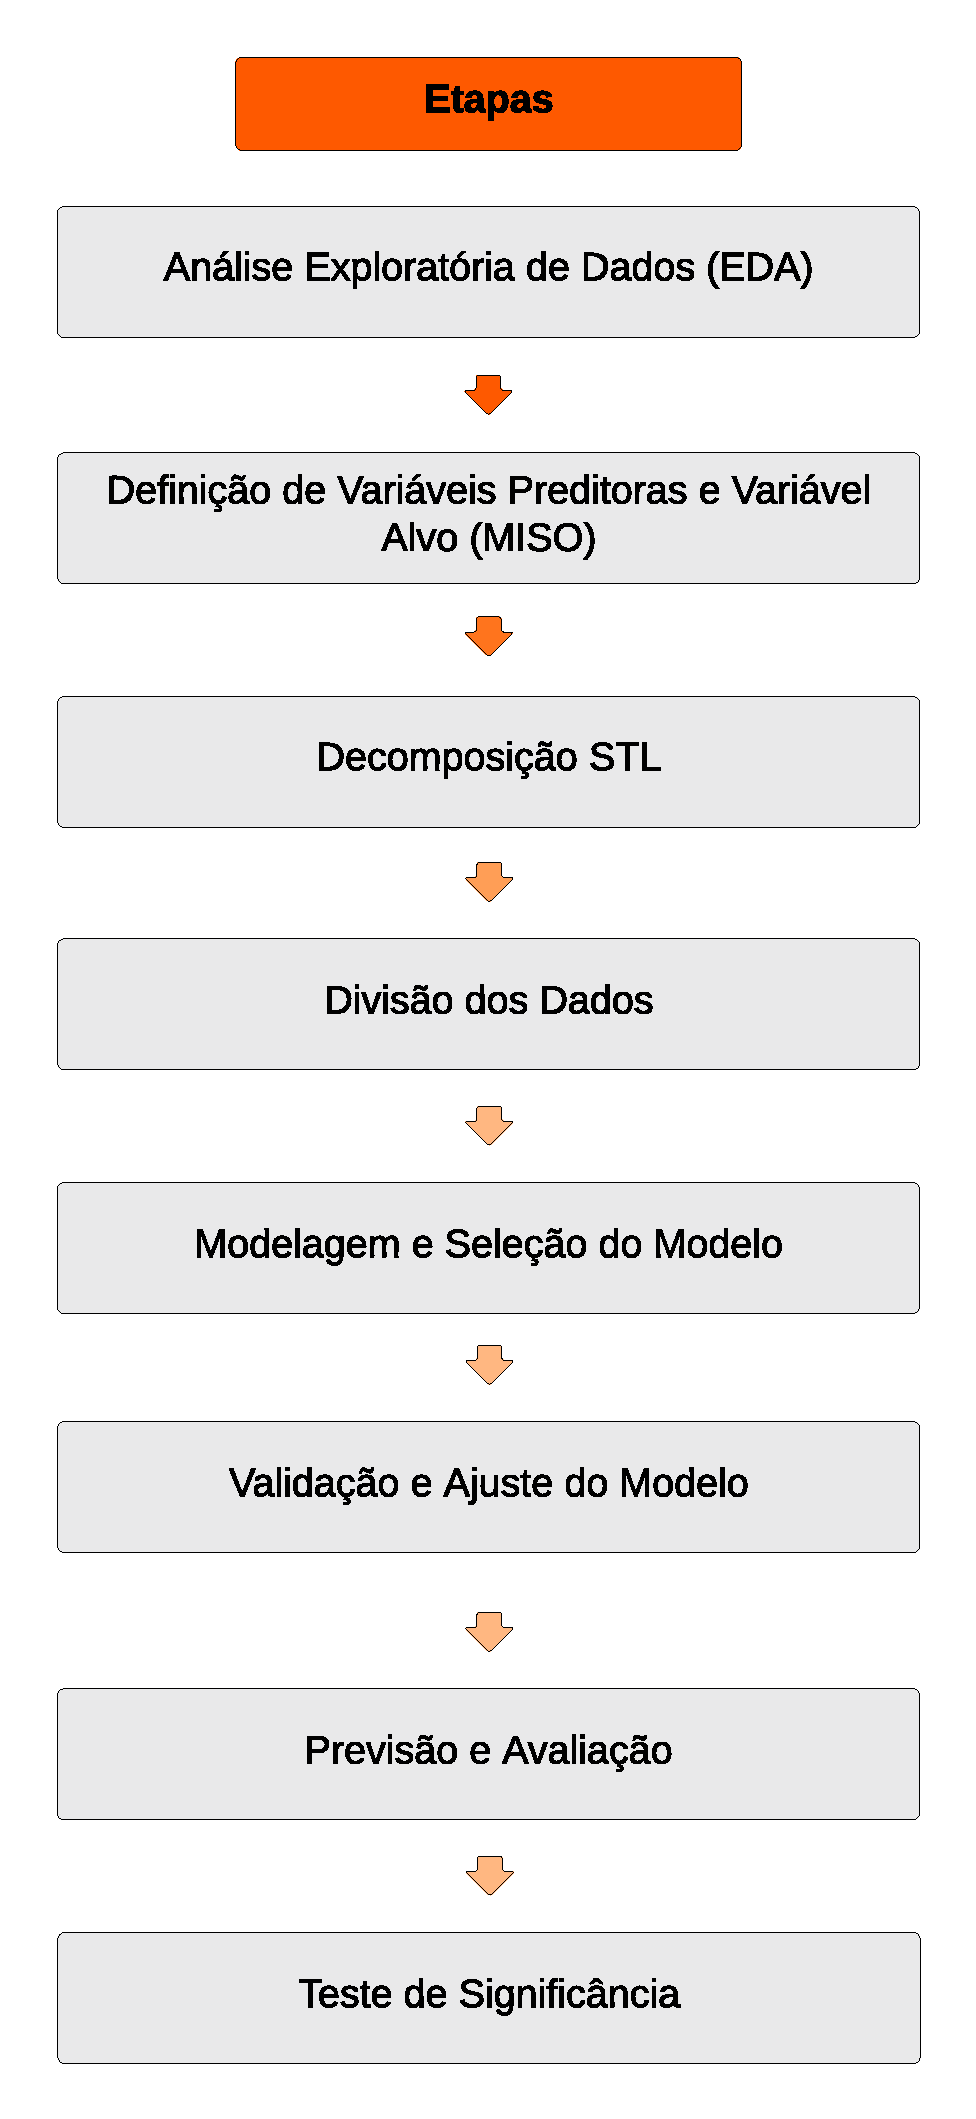
\includegraphics[width=0.7\linewidth]{Introducao/Figuras/Etapas}
	
	
\end{figure}

\noindent As etapas da pesquisa incluem:
\begin{enumerate}[start=1, label={\textbf{Etapa} \arabic*}]
	
	\item \label{etp:1} \textbf{Análise Exploratória de Dados (EDA)}: Nesta etapa  tem-se a identificação de valores ausentes, a observação de padrões temporais e a detecção de anomalias. Gráficos de linha são comuns para visualizar a convergência dos dados \cite{Rostam2021108249}.
	
	\item \label{etp:2} \textbf{Definição de Variáveis Preditoras e Variável Alvo (MISO)}: Na segunda etapa, as variáveis preditoras e a variável alvo para a previsão de Múltiplas Entradas e Uma Saída (do inglês\textit{ Multiple Inputs Single Output}, MISO) são selecionadas. Diferentes modelos, podem incorporar variáveis exógenas na modelagem. Essas variáveis exógenas aprimoram as capacidade de previsão do modelo, especialmente quando o horizonte de previsão se estende além dos dados históricos \cite{PAWLOWSKI202298}. 
	
	\item \label{etp:3} \textbf{Decomposição STL}: O método de decomposição STL (do inglês \textit{Seasonal and Trend Decomposition Using locally estimated scatterplot smoothing (Loess)}) separa uma série temporal em três componentes: sazonalidade, tendência e resíduo. Essa decomposição permite. Decompor séries temporais em sazonal captura variações periódicas e repetitivas. Decompor séries temporais em tendência reflete a evolução geral dos dados ao longo do tempo. Já a componente de resíduo engloba as variações não explicadas pelas anteriores \cite{Bandara2021}.
	
	\item \label{etp:4} \textbf{Divisão dos Dados}: É prática comum dividir o conjunto de dados em conjuntos de treinamento, validação e teste para avaliar o desempenho do modelo. Essa divisão permite uma análise da capacidade de generalização dos modelos, evitando problemas de ajuste excessivo ou insuficiente. A proporção de alocação pode variar, mas uma abordagem é alocar 70\% para treinamento e validação, e os 30\% restantes para o conjunto de testes. A porção de treinamento e validação pode ser subdividida em 80\% para treinamento e 20\% para validação \cite{Tao2020}.
	
	\item \label{etp:5} \textbf{Modelagem e Seleção do Modelo}: Nesta etapa, diversos modelos são construídos e avaliados. Alguns modelos comumente usados para previsão de séries temporais incluem ARX, AR, MA, ARIMA, SARIMA, SARIMAX  e modelos de aprendizado de máquina como RNN, LSTM, GRU, Transformer (Transformador), DTR (do inglês \textit{Decision tree regressor}), LR (do inglês \textit{Linear Regression}), XGBoost (do inglês \textit{eXtreme Gradient Boosting}), Light GBM além do Prophet. A escolha do modelo baseia-se em critérios como desempenho na validação, simplicidade do modelo e interpretabilidade dos resultados.
	
	\item \label{etp:6} \textbf{Validação e Ajuste do Modelo}: Durante a construção do modelo, é importante avaliar seu desempenho usando dados de validação. Neste contexto, métricas de avaliação tais como de avaliação como MAE (Erro Médio Absoluto), sMAPE (Erro Médio Percentual Absoluto Simétrico) e RRMSE (Raiz do Erro Médio Quadrático Relativo) podem ser usadas para comparar e selecionar o melhor modelo. Além disso, técnicas de ajuste como otimização de hiperparâmetros e refinamento do modelo usando dados de treinamento e validação combinados podem melhorar o desempenho de previsão de séries temporais.
	
	\item \label{etp:7} \textbf{Previsão e Avaliação}: Com o modelo final com os dados de treinamento e validação, é possível fazer previsões para o conjunto de testes, que representa dados futuros não observados. Essas previsões são comparadas com os valores reais correspondentes para avaliar a qualidade e precisão do modelo.
	
	\item \label{etp:8} \textbf{Teste de Significância}: Aplicar os modelos de previsão e fazer comparativo baseado em testes de significância estatística (\textit{Friedman e Nemenjy}).
	
	O teste de Friedman é uma ferramenta estatística não paramétrica utilizada para comparar três ou mais grupos relacionados quando os dados não atendem aos pressupostos da ANOVA. Ele determina se há diferenças significativas entre os grupos. Se a diferença for confirmada, o teste de Nemenyi é frequentemente empregado para realizar comparações múltiplas entre grupos específicos, identificando quais pares são significativamente diferentes após a rejeição da hipótese nula no teste de Friedman. Assim, esses métodos são cruciais quando se deseja comparar múltiplos grupos sem fazer suposições sobre a distribuição dos dados.
	
	
\end{enumerate}

Cada uma dessas etapas desempenha um papel crucial na pesquisa e no processo de modelagem de séries temporais, contribuindo para a compreensão dos dados, construção e validação dos modelos.


\subsection{Justificativa da Pesquisa} \label{subsec:justif}

Ao longo desta dissertação, os seguintes aspectos são abordados visando a previsão e tomada de decisões.

\subsubsection{Contribui\c c\~oes} \label{subsubsec:Contribuição}


A dissertação fundamenta-se em modelos previamente não explorados neste contexto, como GRU, LSTM, XGBOOST, LGBM, Transformer, RNN, ANN e CNN. A primeira contribuição aborda a previsão da demanda de água em Curitiba, considerando elementos como consumo e consumo de energia durante picos.

Vários desses modelos na literatura não foram aplicados neste tema de demanda de água, utilizando-os para comparação entre si e em relação aos modelos que já foram trabalhados nesse contexto de demanda d'água, a fim de certificar se esses modelos podem ou não ser utilizados nesse contexto.

Os modelos do tipo ARIMA e suas variantes foram aplicados neste tema, como demonstrado por \cite{2-s2.0-85069459067, 2-s2.0-85099424908}. Alguns outros modelos, apesar de suas vantagens, ainda não foram devidamente aplicados, como é o caso do modelo de RNN \cite{2-s2.0-85067419084}, que se mostrou significativamente superior aos outros 19 modelos listados ao longo deste trabalho.

\subsection{Estrutura da Disserta\c c\~ao} \label{subsec:estrutura}


Essa dissertação está organizada em capítulos. Cada um abordando aspectos específicos da pesquisa. 
O Capítulo~\ref{sec:int},  apresentou uma contextualização do estudo, destacando a motivação e os objetivos a serem alcançados. 

O Capítulo~\ref{sec:refteo}, menciona uma visão geral das principais pesquisas.

No Capítulo~\ref{sec:base}, são apresentados os modelos que serão utilização dos dados de séries temporais da SANEPAR, com os dados coletados.


O Capítulo~\ref{sec:result}, apresenta os resultados obtidos ao longo da pesquisa.  Os resultados de previsão são detalhados, evidenciando análises quanto aos modelos de previsão projetados.

Finalizando, o Capítulo~\ref{sec:conclusoes} apresenta os resultados da pesquisa.



\begin{figure}[!htb]
	\centering
	\caption{Estrutura da dissertação}
	\label{fig:estrutura}
	\includegraphics[width=0.75\linewidth]{Introducao/Figuras/estrutura}
	
	
\end{figure}

